\paragraph{}
A polyhedral cell can be regarded as one of the subdomain\hl{s} in the SBFEM as plotted in Fig.~\ref{oct_fig:sbfem_intro}.
Similar to SBFEM in 2D which has been introduced in Sec.~\ref{iso_section:formulation}, only the boundary surface requires discretization and a scaling center $O$ located at the place where all boundary surfaces of the subdomain are visible is necessary.
%
\begin{figure}
    \centering
    \begin{subfigure}[b]{0.48\linewidth}
        \scalebox{0.5}{
            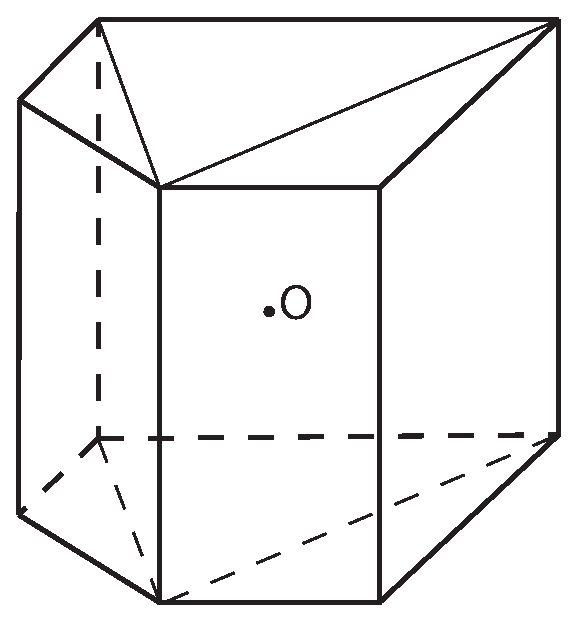
\includegraphics{octree/images/sbfem3d.eps}
        }
        \caption{Scaling center located inside of the subdomain}
        \label{oct_fig:sbfem_intro_a}
    \end{subfigure}
    \begin{subfigure}[b]{0.48\linewidth}
        \scalebox{0.5}{
            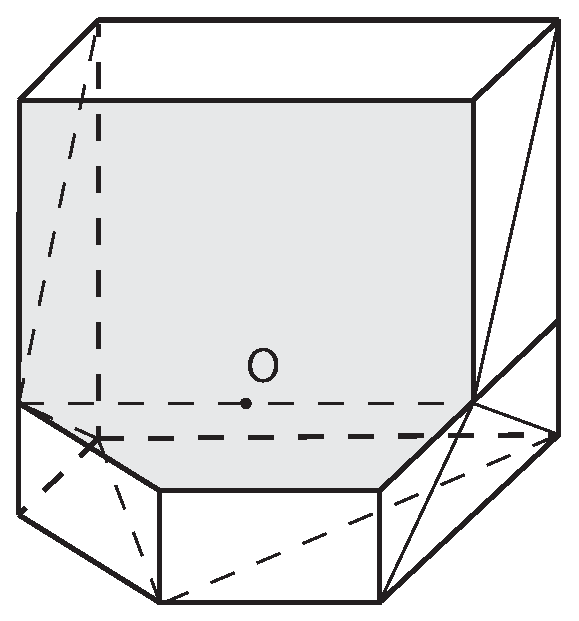
\includegraphics{octree/images/sbfem3d_b.eps}
        }
        \caption{Scaling center located on one of the edges}
        \label{oct_fig:sbfem_intro_b}
    \end{subfigure}
    \caption[Polyhedral SBFEM subdomain in 3D]{Polyhedral subdomain in SBFEM}
    \label{oct_fig:sbfem_intro}
\end{figure}
%
A scaling center on the edge as shown in Fig.~\ref{oct_fig:sbfem_intro_b} is also valid which increases the flexibility and allow\hl{s} the concave subdomain.
In this situation, the triangulated faces containing the scaling center will not be discretized.

\paragraph{}
The transformation between SBFEM coordinate $(\xi, \eta, \zeta)$ and Cartesian coordinate $(x, y, z)$ can be derived from Eq.~\ref{lr_eq:sbfem_boundary_interpolate} and Eq.~\ref{lr_eq:sbfem_scaling} as:
\begin{subequations}
\begin{align}
    x(\xi, \eta, \zeta) & = \xi \hat{x}(\eta, \zeta)  = \xi \mathbf{N}(\eta, \zeta) \mathbf{\hat{x}} \\
    y(\xi, \eta, \zeta) & = \xi \hat{y}(\eta, \zeta)  = \xi \mathbf{N}(\eta, \zeta) \mathbf{\hat{y}} \\
    z(\xi, \eta, \zeta) & = \xi \hat{z}(\eta, \zeta)  = \xi \mathbf{N}(\eta, \zeta) \mathbf{\hat{z}}
\end{align}
\end{subequations}
%
where $(\hat{x}, \hat{y}, \hat{z})$ stands for the point in Cartesian coordinate on the boundary, $(\mathbf{\hat{x}}, \mathbf{\hat{y}}, \mathbf{\hat{z}})$ represents the nodal coordinate vectors and $\mathbf{N}$ is the shape function.
The corresponding Jacobian matrix in 3D on the boundary $(\xi = 1)$ can be expressed as:
\begin{equation}
    \mathbf{J} (\eta, \zeta) =
    \begin{bmatrix}
        x(\eta, \zeta)      &   y(\eta, \zeta)      &   z(\eta, \zeta)  \\
        x(\eta, \zeta),_{\eta}      &   y(\eta, \zeta),_{\eta}      &   z(\eta, \zeta),_{\eta}  \\
        x(\eta, \zeta),_{\zeta}      &   y(\eta, \zeta),_{\zeta}      &   z(\eta, \zeta),_{\zeta}  \\
    \end{bmatrix}
\end{equation}
%
and the displacement interpolation in Eq.~\ref{lr_eq:sbfem_disp_interpolation} becomes
\begin{equation}
    \mathbf{u}(\xi, \eta, \zeta) = \mathbf{N} (\eta, \zeta) \mathbf{u} (\xi)
\end{equation}
%
The linear operator in Eq.~\ref{lr_eq:sbfem_l_operator} becomes
\begin{equation}
    \mathbf{L} = \mathbf{b}_1 (\eta, \zeta) \frac{\partial}{\partial \xi} +
    \frac{1}{\xi}\left(
        \mathbf{b}_2 (\eta, \zeta) \frac{\partial}{\partial \eta} +
        \mathbf{b}_3 (\eta, \zeta) \frac{\partial}{\partial \zeta}
    \right)
\end{equation}
%
Little $b$ matrix in Eq.~\ref{lr_eq:sbfem_little_b} becomes
\begin{subequations}
\begin{align}
    \mathbf{b}_1 (\eta, \zeta) &= \frac{1}{|\mathbf{J}|}
    \begin{bmatrix}
        y,_{\eta} z,_{\zeta} - z,_{\eta} y,_{\zeta} & 0 & 0 \\
        0 & z,_{\eta} x,_{\zeta} - x,_{\eta} z,_{\zeta} & 0 \\
        0 & 0 & x,_{\eta} y,_{\zeta} - y,_{\eta} x,_{\zeta} \\
        0 & x,_{\eta} y,_{\zeta} - y,_{\eta} x,_{\zeta} & z,_{\eta} x,_{\zeta} - x,_{\eta} z,_{\zeta} \\
        x,_{\eta} y,_{\zeta} - y,_{\eta} x,_{\zeta} & 0 & y,_{\eta} z,_{\zeta} - z,_{\eta} y,_{\zeta} \\
        z,_{\eta} x,_{\zeta} - x,_{\eta} z,_{\zeta} & y,_{\eta} z,_{\zeta} - z,_{\eta} y,_{\zeta} & 0
    \end{bmatrix} \\
    \mathbf{b}_2 (\eta, \zeta) &= \frac{1}{|\mathbf{J}|}
    \begin{bmatrix}
        y,_{\zeta} z - z,_{\zeta} y & 0 & 0 \\
        0 & z,_{\zeta} x - x,_{\zeta} z & 0 \\
        0 & 0 & x,_{\zeta} y - y,_{\zeta} x \\
        0 & x,_{\zeta} y - y,_{\zeta} & z,_{\zeta} x - x,_{\zeta} z \\
        x,_{\zeta} y - y,_{\zeta} & 0 & y,_{\zeta} z - z,_{\zeta} y \\
        z,_{\zeta} x - x,_{\zeta} z & y,_{\zeta} z - z,_{\zeta} y & 0
    \end{bmatrix} \\
    \mathbf{b}_3 (\eta, \zeta) &= \frac{1}{|\mathbf{J}|}
    \begin{bmatrix}
        y z,_{\eta} - z y,_{\eta} & 0 & 0 \\
        0 & z x,_{\eta} - x z,_{\eta} & 0 \\
        0 & 0 & x y,_{\eta} - y x,_{\eta} \\
        0 & x y,_{\eta} - y x,_{\eta} & z x,_{\eta} - x z,_{\eta} \\
        x y,_{\eta} - y x,_{\eta} & 0 & y z,_{\eta} - z y,_{\eta} \\
        z x,_{\eta} - x z,_{\eta} & y z,_{\eta} - z y,_{\eta} & 0
    \end{bmatrix}
\end{align}
\end{subequations}
%
Follow the same manner in Sec.~\ref{iso_section:formulation}, the strains can be expressed as
\begin{equation}
    \epsilon(\xi, \eta, \zeta) =
    \mathbf{B}_1 (\eta, \zeta) \mathbf{u} (\xi),_\xi +
    \frac{1}{\xi} \mathbf{B}_2 (\eta, \zeta) \mathbf{u} (\xi)
\end{equation}
%
where
\begin{subequations}
\begin{align}
    \mathbf{B}_1 (\eta, \zeta) & =
    \mathbf{b}_1 (\eta, \zeta) \mathbf{N} (\eta, \zeta) \\
    \mathbf{B}_2 (\eta, \zeta) & =
    \mathbf{b}_2 (\eta, \zeta) \mathbf{N} (\eta, \zeta),_\eta +
    \mathbf{b}_3 (\eta, \zeta) \mathbf{N} (\eta, \zeta),_\xi
\end{align}
\end{subequations}
%
The stress in Eq.~\ref{lr_eq:sbfem_stress} becomes
\begin{equation}
    \sigma(\xi, \eta, \zeta) = \mathbf{D} \left(
        \mathbf{B}_1 (\eta, \zeta) \mathbf{u} (\xi),_\xi +
        \frac{1}{\xi} \mathbf{B}_2 (\eta, \zeta) \mathbf{u} (\xi)
    \right)
\end{equation}
%
and the ODE equation in Eq.~\ref{lr_eq:sbfem_ODE} becomes
\begin{equation}
    \mathbf{E}_0 \xi^2 \mathbf{u}(\xi),_{\xi\xi} +
    (2\mathbf{E}_0 + \mathbf{E}_1^T - \mathbf{E}_1)\xi \mathbf{u}(\xi),_{\xi} -
    (\mathbf{E}_1^T - \mathbf{E}_2) \mathbf{u}(\xi)
    = 0
\label{oct_eq:sbfem_ode}
\end{equation}
%
The coefficient matrices $\mathbf{E}_0$, $\mathbf{E}_1$ and $\mathbf{E}_2$ for element $e$ are expressed as
\begin{subequations}
\begin{align}
    \mathbf{E}_0 = \int_e \mathbf{B}_1^T \mathbf{D} \mathbf{B}_1 |\mathbf{J}| d\eta d\zeta \\
    \mathbf{E}_1 = \int_e \mathbf{B}_2^T \mathbf{D} \mathbf{B}_1 |\mathbf{J}| d\eta d\zeta \\
    \mathbf{E}_2 = \int_e \mathbf{B}_2^T \mathbf{D} \mathbf{B}_2 |\mathbf{J}| d\eta d\zeta 
\end{align}
\end{subequations}
%
The internal nodal forces $\mathbf{q}(\xi)$ on the boundary can be determined as \citep{Son2004a}
\begin{equation}
    \mathbf{q} (\xi) = \xi (
        \mathbf{E}_0 \xi \mathbf{u}(\xi),_\xi +
        \mathbf{E}_1^T \mathbf{u}(\xi)
    )
\label{oct_eq:sbfem_nodal_forces}
\end{equation}
%
$X(\xi)$ is introduced to reduce the order of the ODE in Eq.~\ref{oct_eq:sbfem_ode} as
\begin{equation}
    \mathbf{X} (\xi) =
    \begin{bmatrix}
        \xi^{0.5} \mathbf{u}(\xi) \\
        \xi^{-0.5} \mathbf{q}(\xi)
    \end{bmatrix}
\label{oct_eq:sbfem_x}
\end{equation}
%
substituting Eq.~\ref{oct_eq:sbfem_x} and Eq.~\ref{oct_eq:sbfem_nodal_forces} into Eq.~\ref{oct_eq:sbfem_ode} yields
\begin{equation}
    \xi \mathbf{X} (\xi),_\xi =
    -\mathbf{Z} \mathbf{X} (\xi)
\end{equation}
%
where $Z$ is the hamiltonian matrix
\begin{equation}
    \mathbf{Z} =
    \begin{bmatrix}
        \mathbf{E}_0^{-1} \mathbf{E}_1^T - 0.5 \mathbf{I}   &   -\mathbf{E}^{-1}_0 \\
        -\mathbf{E}_2 + \mathbf{E}_1 \mathbf{E}_0^{-1} \mathbf{E}_1^T   &   -(
            \mathbf{E}_1 \mathbf{E}_0^{-1} - 0.5 \mathbf{I}
        )
    \end{bmatrix}
\label{oct_eq:sbfem_z}
\end{equation}
%
An eigenvalue decomposition of Eq.~\ref{oct_eq:sbfem_z} is performed and it yields
\begin{equation}
    \mathbf{X} (\xi) =
    \begin{bmatrix}
        \Phi_{u1}   &   \Phi_{u2} \\
        \Phi_{q1}   &   \Phi_{q2}
    \end{bmatrix}
    \begin{bmatrix}
        \xi^{-\lambda}  &   0 \\
        0   &   \xi^{\lambda}
    \end{bmatrix}
    \begin{bmatrix}
        \mathbf{c}_1  &   0   \\
        0   &   \mathbf{c}_2
    \end{bmatrix}
\label{oct_eq:sbfem_eigenvalue}
\end{equation}
%
where $\pm\lambda$ is the eigenvalue and $-\lambda$ is corelate to the real parts.
$\Phi$ is part of the matrix of the eigenvector matrix.
$\mathbf{c}_1$ and $\mathbf{c}_2$ stand for the integration constant.
Modal displacements and forces in Eq.~\ref{lr_eq:sbfem_general_sol_str} becomes
\begin{subequations}
\begin{align}
    \mathbf{u}(\xi) &= \mathbf{\Phi}_{u1} \xi^{-\Lambda-0.5\mathbf{I}} \mathbf{c}_1
    \label{oct_eq:sbfem_general_sol_disp} \\
    \mathbf{q}(\xi) &= \mathbf{\Phi}_{q1} \xi^{-\Lambda+0.5\mathbf{I}} \mathbf{c}_2
    \label{oct_eq:sbfem_general_sol_str}
\end{align}
\end{subequations}
%
The stiffness matrix then can be derived as
\begin{equation}
    \mathbf{K} = \Phi_{q1} \Phi_{u1}^{-1}
\end{equation}